\documentclass{article}
\usepackage[utf8]{inputenc}
\usepackage[american]{babel}
\usepackage[T1]{fontenc}
\usepackage{amssymb,amsthm,amsmath,amsfonts}
\usepackage{algorithmic}
\usepackage{algorithm}
\usepackage{tikz}
\usepackage{nicefrac}
 
\newcommand{\todo}[1]{{\color{red}TODO: #1}}

\theoremstyle{plain}
\newtheorem{thm}{Theorem}
\newtheorem{lem}[thm]{Lemma}
\newtheorem{cor}[thm]{Corollary}
\newtheorem{prop}[thm]{Proposition}
\theoremstyle{definition}
\newtheorem{defi}[thm]{Definition}
\theoremstyle{remark}
\newtheorem{rem}[thm]{Remark}
\newtheorem{exe}[thm]{Example}

\title{Explicit isogenies in quadratic time in any characteristic}
\author{Cyril Hugounenq}

\begin{document}

\maketitle

\begin{abstract}
The problem we will consider here is the computation of an isogeny between two elliptics curves with the knowledge of the domain and the codomain of the isogeny and it's degree $r$. Couveignes's algorithm is an algorithm which solves this problem in $O(r^2)$ operations using the $p$-torsion. We want to extend the method used by Couveignes  We try to adapt his method here to the case of the $2$ torsion and more generally to the $\ell$ torsion, thus we propose an alternative for medium characteristic with this algorithm.
\end{abstract}

\section*{Proposed notation}

This section is for internal reference only: erase after the paper has
stabilized.

\begin{itemize}
\item $\mathbb{F}_q$ is the field we are working on
\item $\ell$ is for the $\ell$ torsion we are working on
\item $r$ is the degree of the isogeny we want to compute
\item $k$ is the integer such that $\ell^{2k}>4r+1$
\item we thus work with a tower which has for top level $F_{q^{\ell^k}}$
\item $E$ is for ordinary elliptic curves defined over the finite field $\mathbb{F}_q$
\item $\mathcal{O}$ (resp. $\mathcal{O}_x$) is the notation for the endomorphism ring associated (up to isomorphism) to $E$ (resp. $E_x$)
\item $K$ is the notation for the imaginary quadratic field in which $\mathcal{O}$ is defined
\item $d_K$ is the negative integer such that $K=\mathbb{Z}[d_K]$  
\end{itemize}

%%%%%%%%%%%%%%%

\section{Introduction}
\label{sec:introduction}

\todo{Isogenies of elliptic curves over finite fields are
  important. Isogenies are used in SEA. Isogenies are used in
  cryptography.  The \emph{explicit isogeny problem} is defined as
  follows\dots It is a fundamental subproblem in SEA. The best
  algorithms for it are\dots We present a quasi-quadratic-time
  algorithm working for finite fields of any characteristic, it is an
  alternative to the Lercier-Sirvent approach and compares favorably
  to it.}

% From a mail by Luca

% - Dans SEA, pour compter le nombre de points sur GF(p^n), on doit
% calculer des isogénies de degre ℓ~log(p^n).

% - Les algos classiques de calcul d'isogénies (CCR et BMSS) ratent dès
% que p >> ℓ.

% - Pour p fixé, on n'utilise pas SEA, mais plutôt les algos p-adiques.
% Ces algos sont exponentiels en log p.

% - Du coup, pour p pas fixé et n >> p/log(p) (carac moyenne), il y
% encore un intérêt à chercher des algos de calcul d'isogénies
% polynômiaux en log p.

% - Le seul algo de calcul d'isogénies qui marche pour tout p et qui
% n'est pas exponentiel en log p est Lercier-Sirvent. Il est quadratique
% en ℓ (plus le coût du polynôme modulaire, qui de toutes façons est
% déjà inclus dans SEA).

% Du coup, même si la carac moyenne n'est pas vraiment utilisée en
% crypto, ça reste intéressant de chercher des algos de calcul
% d'isogénie pour concurrencer Lercier-Sirvent.

The paper is organized as follows. In Section~\ref{sec:couv-algor} we
review Couveignes' strategy for the explicit isogeny problem, and
sketch our generalization of it. In
Section~\ref{sec:isogeny-volcanoes} we recall the fundamental
properties of isogenies and endomorphism
rings. Sections~\ref{sec:acti-frob-endm} and~\ref{sec:interpolation}
treat the two main phases of our new algorithm; both phases are used
together in Section~\ref{sec:complete-algorithm} to give the full
algorithm. Finally, Section~\ref{sec:implem} describes our
implementation of the algorithm and discusses its performances.


%%%%%%%%%%%%%%%

\section{Couveignes' algorithm}
\label{sec:couv-algor}

%Rappel sur l'algorithme de Couveignes, dire que basiquement il interpole un groupe de points sur un autre, puis fait de la reconstruction rationnelle et teste alors si son résultat est correct, si ce n'est pas le cas il change les groupes et recommence. 

Couveignes' algorithm \cite{couveignes96} is an algorithm which computes an isogeny using the $p$-torsion. This algorithm takes advantage of the cyclic group structure of the $p$ torsion to interpolate $p^k$ torsion points of one curve on another, with $k$ chosen such that $p^k>4r$. Couveignes's algorithm also take into account that if an isogeny send a point on an other then it also must respect the same property for the multiple points. With the interpolation polynomial Couveignes do a rational reconstruction of the isogeny, if the rational reconstruction don't work he tried with another couple of generators to do another interpolation. The complexity of this algorithm is of $O(r^2)$
\newline
We adapt his method here to the case of the $2$ torsion for ordinary elliptic curves and more generally to the $\ell$ torsion with $2 \wedge r ( \ell \wedge r)$.

Our goal is to reduce the number of points to interpolate with operations which are not so much costly. Thus we consider the Frobenius endomorphism to give us knowledge on the points we want to interpolate. We have considered the graph of isogeny (called volcano) which is linked to the group structure (see \cite{MiretMRV05}, \cite{IonicaJ10} ) of the curve for our study. First we have to determined which knowledge we obtain thanks to the Frobenius. The Frobenius allow us to determine horizontal isogenies according to the "notations" from \cite{Kohel} and \cite{volcano}, and thus we can associate to those horizontal isogenies their kernel and then one generator of their kernel. It will be those generators that we will use for the interpolation. To speed up the interpolation computation we will use techniques such as one used in \cite{enge+morain03} where we take into account the action of the Frobenius. In the end we will obtain a computational complexity of $O(r^2)$.

%%%%%%%%%%%%%%%

\section{Isogeny volcanoes}
\label{sec:isogeny-volcanoes}

\todo{Notions de base sur les isogenies et les volcans.}

%Dire que le volcan ne possède des isogenies
\subsection{ordres sur les corps quadratiques}%titre a supprimer eventuellement
We will denote by $\mathcal{O}$ (resp. $\mathcal{O}_i$) the endomorphism ring associated up to isomorphism to the elliptic curve $E$ (resp. $E_i$). As we work only with ordinary elliptic curves, we recall that $\mathcal{O}$ is an order in a quadratic imaginary field usually denoted by $K$. The maximal order (and algebraic integers of $K$) is denoted by $\mathcal{O}_K$ and we denote its discriminant by $d_K$, we remind that $\mathcal{O}_K=\mathbb{Z}[\frac{d_K+\sqrt{d_K}}{2}]$. For every order $\mathcal{O}$ in $K$ we have the following results : $\mathcal{O}= \mathbb{Z}+ f \mathcal{O}_K$ with the conductor $f=[\mathcal{O}:\mathcal{O}_K]$ and the discriminant $D=f^2d_K$. For more detailed informations we refer the reader to \cite{Cox89}. We need also to reminde that for an odd prime $\ell$ we have the Legendre symbol $\left( \frac{d_K}{\ell} \right)=$ and for $\ell=2$ we have the Kronecker symbol $\left( \frac{d_K}{2} \right)= 1$ if $d_K = 1 \bmod 8$, $\left( \frac{d_K}{2} \right)= -1$ if $d_K = 5 \bmod 8$ and $\left( \frac{d_K}{2} \right)= 0$ if $2 \mid d_K$ %derniere ligne a mieux remettre en forme


\subsection{Isogenies montantes- descendantes}
We remind a result from Kohel \cite{Kohel} for the endomorphism rings of ordinary elliptic curves:
\begin{prop}
Let $\phi:E \rightarrow E'$ be an isogeny of degree $\ell$. Then 
\begin{itemize}
\item $\phi$ is an ascending isogeny if we have $[\mathcal{O}:\mathcal{O'}]=\ell$,
\item $\phi$ is a descending isogeny if we have $[\mathcal{O'}:\mathcal{O}]=\ell$,
\item $\phi$ is an horizontal isogeny if we have $[\mathcal{O'}:\mathcal{O}]=1$.
\end{itemize}
\end{prop}
We call an isogeny of degree $\ell$ a $\ell$ isogeny.
We denote by $\pi$ the Frobenius morphism, it is an endomorphism as like the scalar multiplications, thus we always have for an elliptic curve $E$:
$\mathbb{Z}[\pi] \subset \mathcal{O} \subset \mathcal{O}_K$.
We consider the Frobenius and his action on the $\ell$ torsion on an elliptic curve $E$, thus it is relevant to consider it's characteristic polynomial on $\mathbb{F}_q$:
\begin{equation}
X^2 - tX +q = 0
\end{equation}
with $t$ the Frobenius trace of the elliptic curve $E$. We denote by $d_{\pi}$ the discriminant of this polynomial it also corresponds to the discriminant associated to the order $\mathbb{Z}[\pi]$. We denote by $\lambda_1$ and $\lambda_2$ when they exist the roots of this polynomial, , and in the next section we  determine "eigenspaces" in the $\ell$ torsion for those "eigenvalues".

\begin{defi}
We define the cost of computing the Frobenius on a finite field of size $q^n$ with the complexity expressed in terms of operations on $\mathbb{F}_q$ by the following function: $F(q,n)$.
\end{defi}

\subsection{Volcan}
We call volcano of $\ell$ isogenies, the graph of $\ell$ isogenies. There are three types of volcano according to the shape of their the top level (crater) in the graph with respect to the vocabulary of ascending and descending isogeny. $\mathcal{O}_K$ is the endomorphism ring associated to the crater (top level) of the volcano. According to the value of $\left( \frac{d_{K}}{\ell} \right)$ (with $\left( \frac{\cdot}{\cdot} \right)$ the Legendre symbol) there are $3$ kind of volcano: with cyclic crater, with crater reduced to one point, with crater reduced to two points. We remind a proposition from \cite{kohel} about the structure of the volcano of $\ell$ isogeny.
\begin{prop} %prop 23 de la these de Kohel
Let $E$ be an elliptic curve with an associated endomorphism ring $\mathcal{O}$ of discriminant $D$, %let $\ell$ be a prime and let $\left( \frac{D}{\ell} \right)$ the Legendre symbol
\begin{itemize}
\item if $\mathcal{O}$ is maximal (i.e. equals to $\mathcal{O}_K$) then there are $\left( \frac{D}{\ell} \right) +1 $ horizontal $\ell$ isogenies,
\item if $\mathcal{O}$ is non maximal then there are no horizontal $\ell$ isogenies,
\item if there exists more than $\left( \frac{D}{\ell} \right) +1 $  $\ell$isogenies, up to isomorphism, then all the isogenies are defined over $\mathbb{F}_q$ and there is only $1$ ascending isogeny. 
\end{itemize}
\end{prop} 


		\begin{figure}
		\begin{center}
		
        \begin{tikzpicture}[scale=0.5]
        \coordinate (A) at (0,0);
		\coordinate (B) at (230:5);
		\coordinate (C) at (270:4);
		\coordinate (D) at (310:5);
		\draw (A) node{$\bullet$};
		\draw (B) node{$\bullet$};
		\draw (C) node{$\bullet$};
		\draw (D) node{$\bullet$};
		\draw (A)--(B);
		\draw (A)--(C);
		\draw (A)--(D);
		
		\begin{scope}[xshift=7cm]
		\coordinate (A) at (0,0);
		\coordinate (B) at (5.5,0);
		\coordinate (C) at (240:4.2);
		\coordinate (D) at (300:4.2);
		\draw (A) node{$\bullet$};
		\draw (B) node{$\bullet$};
		\draw (C) node{$\bullet$};
		\draw (D) node{$\bullet$};
		\draw (A)--(B);
		\draw (A)--(C);
		\draw (A)--(D);
		\end{scope}
		
		\begin{scope}[xshift=12.5cm]
		\coordinate (A) at (0,0);
		\coordinate (C) at (240:4.2);
		\coordinate (D) at (300:4.2);
		\draw (A) node{$\bullet$};
		\draw (C) node{$\bullet$};
		\draw (D) node{$\bullet$};
		\draw (A)--(C);
		\draw (A)--(D);
		\end{scope}
		
		\begin{scope}[xshift=23cm]
		\node (A) at (-3,0) {$\bullet$};
		\node (B) at (3,0) {$\bullet$};
		\node (C) at (270:1.2) {$\bullet$};
		\node (D) at (90:1.5) {};
		%\draw[-] (A.center) to[bend right=25] (C.center);
		\draw[-,dashed] (A.center) to[bend left=40] (B.center);
		%\draw[-] (B.center) to[bend left=25] (C.center);
		%\draw[-,dashed] (B.center) to[bend right] (D.center);
		\draw[-] (A.center) to[bend right=40] (B.center);
			\begin{scope}[xshift=-3cm]
			\coordinate (A) at (0,0);
			\coordinate (C) at (270:4.2);
			\draw (A) node{$\bullet$};
			\draw (C) node{$\bullet$};
			\draw (A)--(C);
			\end{scope}
			\begin{scope}[xshift=3cm]
			\coordinate (A) at (0,0);
			\coordinate (C) at (270:4.2);
			\draw (A) node{$\bullet$};
			\draw (C) node{$\bullet$};
			\draw (A)--(C);
			\end{scope}
			\begin{scope}[yshift=-1.2cm]
			\coordinate (A) at (0,0);
			\coordinate (C) at (270:4.2);
			\draw (A) node{$\bullet$};
			\draw (C) node{$\bullet$};
			\draw (A)--(C);
			\end{scope}
		\end{scope}
		\end{tikzpicture}
		%\end{center}
		\caption{ $3$ kind of volcanos of $2$ isogenies }
		
		\end{center} 
		\end{figure}
	
During the rest of this paper we consider only volcano with cyclic crater (i.e. when $\left( \frac{d_K}{\ell} \right) =1$).

%%%%%%%%%%%%%%%

\section{The action of the Frobenius endmorphism}
\label{sec:acti-frob-endm}
\todo{Dans cette section on montre les résultats que nous permettent d'obtenir le frobenius sur le cratère}
To be able to distinguish two different horizontal isogenies and the descending ones on the crater of the volcano, we need the Frobenius to have two distincts eigenvalues defined on the $\ell$ torsion which is only possible on the cyclic crater of a volcano of $\ell$-isogeny.

\begin{prop}
$\lambda_1 , \lambda_2$ the $2$ eigenvalues of the Frobenius are only defined on the $\ell$ torsion of a curve that is located at the top of a cyclic volcano of $\ell$ isogeny.
\end{prop}

\begin{proof}
We remind that $D=g^2d_K$, with $d_K$ squarefree.
\newline
If we have $\left( \frac{d_K}{\ell} \right)=1$ then we have $x^2 = d_K \bmod \ell$ that has a solution so the characteristic polynomial of the Frobenius has two roots in $\mathbb{Z}_{\ell}$. If $\left( \frac{d_K}{\ell} \right)=-1$ then we have $x^2 = d_K \bmod \ell$ that has no solution so the characteristic polynomial of the Frobenius has no roots in $\mathbb{Z}_{\ell}$. If $\left( \frac{d_K}{\ell} \right)=0$ then we have $x^2 = d_K \bmod \ell$ that has the trivial solution so the characteristic polynomial of the Frobenius has a unique root in $\mathbb{Z}_{\ell}$.
\newline
We thus work with $\left( \frac{d_K}{\ell} \right)=1$. We are obliged to work in $\mathcal{O}_K$ (crater)  since the eigenvalues of the Frobenius are not defined in $\ell^i \mathcal{O}_K$ modulo the $\ell$ torsion for $i>0$ because the discrimant is $D=\ell^2i d_K$ and $\left( \frac{\ell^2 d_K}{\ell} \right)=0$.
\end{proof}

\begin{defi}
For $\lambda_1$, $\lambda_2$ the $2$ distinct eigenvalues of the Frobenius, we define $h=\nu_{\ell} \left( \lambda_1 - \lambda_2 \right)$
\end{defi}

From this point we study the $\ell$ torsion points that are eigenvector for the Frobenius, thus we work in this section only with curves that are on the cyclic crater of a volcano (i.e. when $\left( \frac{d_K}{\ell} \right)=1$). We have to determine  the two eigenvalues of the Frobenius and $2$ points of $\ell^{h+1}$ order who are also eigenvector for the $2$ eigenvalues. First we describe an algorithm to compute the pre image of a point by the multiplication by $\ell$. Then we present an algorithm that computes recursively for $s=1$ to $s=k$ with $k>h$ a basis of the $\ell^s$ torsion with each generator a different eigenvector for the value $\lambda_1, \lambda_2 \bmod \ell^s$.
%First we have to tell how we obtain such a basis and the eigenvalues

\begin{algorithm}
\caption{\label{ldivision}Compute the pre image of $Q$ by the multiplication by $\ell$.}
\begin{algorithmic}[5]
\REQUIRE  $E: y^2=h(x)$ such that $E[\ell] \subset E(\mathbb{F}_q)$ % a reformuler
\STATE $Q$ a point on $E$
\ENSURE $Q/\ell$ such that $\ell(Q/\ell)=Q$
\STATE $ \langle P_1,P_2 \rangle = E[\ell] \gets E $
\STATE $\phi_1  \gets \lbrace E\rightarrow \nicefrac{E}{P_1}=E_1 \rbrace $
\STATE $\phi_2  \gets \lbrace E_1\rightarrow {E_1}/{\phi_1(P_2)}=E \rbrace $
%\STATE $f(x) \gets \phi_2(x)[0]$
%\STATE $P_1(x)=ax^2+bx+c=0 \gets \phi_2(x)[0]=Q[0]$
\STATE $x_1 \gets \phi_2(x_1)[0]=Q[0] $
%\STATE $g(x) \gets \phi_1(x)[0]$
%\STATE $P_2(x)=a_2x^2+b_2x+c_2=0 \gets \phi_1(x)[0]=x_1$
\STATE $x_2 \gets \phi_1(x_2)[0]=x_1  $
%\STATE $h(x)  \gets E $
%\STATE $y_2 \gets y_2^2=h(x_2) $
\RETURN $Q/\ell=(x_2,\sqrt{h(x_2)})$
\end{algorithmic}
\end{algorithm}

\begin{prop}
Algorithm $\ref{ldivision}$ has a complexity for
\begin{enumerate}
\item[$\ell = 2$] of $O(M(\sqrt{r})(\log(r)+\log(q)))$ operations in $\mathbb{F}_q$ ,
\item[$\ell \neq 2$]of $O(\sqrt{r} \log(q) M(\sqrt{r})\log(r))$ operations in $\mathbb{F}_q$.
\end{enumerate}
 
\end{prop}

\begin{proof}
\begin{enumerate}
\item[$\ell = 2$]
The $2$ isogeny generated by a $2$ torsion point is computed according to Velu's formula.
The computation of a $2$ isogeny from its kernel is done in $O(M(2^k))=O(M(\sqrt{r}))$ operations in $\mathbb{F}_q$, the bottle neck is the inversion which is done with this complexity using Newton-Raphson's algorithm.
\newline
Computing the $2$ torsion points of $E$ is done through the calculation of roots of $h(x)$.
Since we consider the input curves has a two torsion of rank $2$ on $\mathbb{F}_q$ we can do the root computation with Cantor-Zassenhauss' algorithm in a complexity of $O( \log(q))$ operations in $\mathbb{F}_q$. 
The computation of a square root is done in $O(M(2^k)\log(2^kq))$ operations in $\mathbb{F}_q$ according to \cite{DBLP:journals/dcc/DoliskaniS15}, thus we have a computational complexity of $O(M(\sqrt{r})(\log(r)+\log(q)))$
\item[$\ell \neq 2$]The computation of a basis of $E[\ell]$ takes $O(\log(q)\ell^6 )$ operations on $\mathbb{F}_q$ using first Cantor-Zassenhauss algorithm to find the points of order $\ell$ and then the Miller algorithm to find  the two generators. Computation of the different abscissas of points in the kernel of the isogeny takes $O(\ell )$ operations on $\mathbb{F}_q$. The cost of the computation of the $\ell$ isogeny is then $O(M(\ell^k)\log(\ell^k))$ operations on $\mathbb{F}_{q}$, the main cost comes from the inverse computation of this complexity according to "\cite{DeDoSc13}". Then we have to find roots of a polynomial of degree $\ell$ (and $2$) in $\mathbb{F}_{q^{\ell^k}}$ which can be done in $O(\log(q^{\ell^k})\ell^3)$ operations on $\mathbb{F}_{q^{\ell^k}}$ using Cantor-Zassenhauss' algorithm thus $O(\log(q^{\ell^k})\ell^3 M(\ell^k)\log(\ell^k))$ operations on $\mathbb{F}_q$. Thus the overall complexity is $O(\sqrt{r} \log(q) M(\sqrt{r})\log(r))$ operations on $\mathbb{F}_q$.
\end{enumerate}
\end{proof}

We restrict ourselves to the case where $E[\ell] \subset E(\mathbb{F}_q)$, because we just have to work in $\mathbb{F}_{q^{\ell-1}}$ to have this hypothesis true. Now we can descirbe the algorithm that computes eigenvalues of the Frobenius $\bmod \ell^k$ and a  basis of the $\ell^{k}$ torsion with each generator an eigenvector for the Frobenius.

\begin{algorithm}
\caption{\label{Diagnoalizedbasis}Diagonalizing and computing the basis $\langle P,Q \rangle $ of the $\ell^k$ torsion.}
\begin{algorithmic}[5]
\REQUIRE $\langle P,Q \rangle$ a basis of the $\ell$-torsion defined on a curve $E$ such that $E[\ell] \subset E(\mathbb{F}_q)$ .
\ENSURE $\langle P,Q \rangle$ a basis of the $\ell^k$-torsion, $\lambda_1, \lambda_2$ defined modulo $\ell^k$ such that $\pi(P)=\lambda_1P$, $ \pi(Q)=\lambda_2Q$
\STATE $h:=1, k_0:=1$
\FOR {$i=1$  to  $k-1$}
\STATE $P \leftarrow P/\ell$
\STATE $Q \leftarrow Q/\ell$ 
\STATE compute $\pi(P,Q)=\left( \begin{array}{cc}
\lambda_1 + a\ell^{i} & b\ell^{i}\\
c\ell^{i} & \lambda_2 + d\ell^{i}
\end{array} \right) \bmod \ell^{i+1}$ with $\{a,b,c,d\} \in \mathbb{Z}/\ell\mathbb{Z}$
\IF {$\lambda_1 \neq \lambda_2$}
\STATE $k0 \leftarrow \frac{\lambda_1-\lambda_2}{\ell^h}$
\ENDIF
\STATE $\lambda_1, \lambda_2  \gets \lambda_1 + a\ell^i, \lambda_2 + d\ell^i$
\STATE $r_1,r_2 \gets \frac{-b }{k_0}, \frac{c }{k_0}$  
\STATE $\{P,Q\} \gets \{P+\ell^{i-1-h}r_1Q,Q+\ell^{i-1-h}r_2P\}$
\IF {$\lambda_1 = \lambda_2$}
\STATE $h \leftarrow h+1$
\ENDIF
\ENDFOR
\RETURN $\{P,Q,\lambda_1,\lambda_2\}$
\end{algorithmic}
\end{algorithm}

\begin{prop}
The computation complexity of algorithm \ref{Diagnoalizedbasis} for 
\begin{enumerate}
\item[$\ell=2$] is of $O((\log(r)^2+\log(q)) M(\sqrt{r}) $ operations in $\mathbb{F}_q$, 
\item[$\ell \neq 2$] is of $O(\sqrt{r} \log(q) M(\sqrt{r})\log^2(r)\log^{-1}(\ell)+ \log(r)\log^{-1}(\ell) F(q,\ell^k))$ operations in $\mathbb{F}_q$.
\end{enumerate}
\end{prop}

\begin{proof}
\begin{enumerate}
\item[$\ell=2$]
Since the complexity of computing the Frobenius is $O(2^k+\log(q))$ operations in $\mathbb{F}_q$ by \cite{DBLP:journals/dcc/DoliskaniS15}, the root computation remains the most costly operation.
\item[$\ell \neq 2$] The cost of computation of ligne $3$ and $4$ is of $O(\sqrt{r} \log(q) M(\sqrt{r})\log(r))$ according to the complexity analysis of algorithm \ref{ldivision}. The cost of the Frobenius is of $F(q,\ell^k)$. The cost of the line 11 is the cost of the $\ell$ multiplication repeated up to $k$ times which is of a complexity similar to the cost of computing an $\ell$ isogeny by using a decomposition of two $\ell$ isogeny. So the overall complexity of line 11 taking into account the for loop is $O(k^2M(\ell^k)\log(\ell^k))=O(M(\sqrt{r}\log(r)^3\log^{-2}(\ell))$. The overall complexity is thus dominated by line $3$ and $4$ with the Frobenius computation, this gave us the following complexity: $O(\sqrt{r} \log(q) M(\sqrt{r})\log^2(r)\log^{-1}(\ell)+ \log(r)\log^{-1}(\ell) F(q,\ell^k)$ on $\mathbb{F}_q$
\end{enumerate}
\end{proof}


To distinguish the two eigenvalues of the Frobenius we have to consider the $\ell^k$ torsion for $k>\nu_{\ell}(\lambda_1-\lambda_2)$. The following result links the $\ell$ isogenies and the $\ell^k$ torsion points.

\begin{prop} \label{conjecture}
For $P$ a point of order $\ell^{h+1}$ on $E$ which is on a cyclic crater, with $\lambda_1, \lambda_2$ the two eigenvalues associated to $\pi$, then
\begin{itemize}
\item Either $\pi(P)=\lambda_1P$ or $\pi(P)=\lambda_2P$ then the $\ell$-isogeny with kernel $\ell^{h} P$ is horizontal,
\item or $\pi(P) \neq \lambda_2P$ and $\pi(P) \neq \lambda_1P$ then the $\ell$-isogeny with kernel $\ell^{h} P$ is descending.
\end{itemize} 
\end{prop}

\begin{proof}
$E_{\lambda_1}=\{P \in E[\ell],  \pi(\frac{P}{\ell^h})=\lambda_1\frac{P}{\ell^h}\}$, $E_{\lambda_2}=\{P \in E[\ell],  \pi(\frac{P}{\ell^h})=\lambda_2\frac{P}{\ell^h}\}$ and consider $\phi_1$(resp. $\phi_2$) the $\ell$isogeny generated by $E_{\lambda_1}$ (resp. $E_{\lambda_2}$).
since we have a cyclic crater $\left( \frac{d_K}{\ell} \right)=1$ then (by Proposition 5.11 of \cite{Cox89} )  $\ell \mathcal{O}_K=\mathfrak{l}_1\mathfrak{l}_2$ with $Gal(K/\mathbb{Q})$ such as $\mathfrak{l}_1'=\mathfrak{l}_2$ (by theorem 5.9 of \cite{Cox89}).
On veut faire pareil en disant que $E_{\lambda_1}=(\ell, \frac{\pi - \lambda_1}{\ell^h})$ idem pour $\lambda_2$, tel que $\ell=(\ell, \frac{\pi - \lambda_1}{\ell^h})(\ell, \frac{\pi - \lambda_2}{\ell^h})$, par un résultat dans Advanced Topics de Silverman, il ne reste plus qu'à prouver que cette décomposition de l'idéal $\ell$ est une décomposition en idéaux premiers. 
%%%%Ancienne preuve avec de très nombreux défauts
%We denote by $E_{\lambda_1}=\{P \in E[\ell^{h+1}], \ell^{h}P \neq 0, \pi(P)=\lambda_1P\}$, $E_{\lambda_2}=\{P \in E[\ell^{h+1}], \ell^{h}P \neq 0, \pi(P)=\lambda_2P\}$ and consider $\phi_1$(resp. $\phi_2$) the $\ell$isogeny generated by $E_{\lambda_1}$ (resp. $E_{\lambda_2}$). This isogeny is unique since those eigenspace are of dimension $1$. % on pourrait se passer de cette dernière phrase... 
%We remind that we have the endomorphism ring of $E$: $\mathcal{O} \subset \mathcal{O}_K $ and $[\mathcal{O}:\mathcal{O}_K] =1$, since we have a cyclic crater $\left( \frac{d_K}{\ell} \right)=1$ then (by Proposition 5.11 of \cite{Cox89} )  $\ell \mathcal{O}_K=\mathfrak{l}_1\mathfrak{l}_2\mathcal{O}_K$ with $Gal(K/\mathbb{Q})$ such as $\mathfrak{l}_1'=\mathfrak{l}_2$ (by theorem 5.9 of \cite{Cox89}). Since $E_{\lambda_1}$ and $E_{\lambda_2}$ are also conjugated with $Gal(K/\mathbb{Q})$ we can associate to the isogeny $\phi_1$ (resp. $\phi_2$)  the integral ideal $\mathfrak{l}_1\mathcal{O}_K$ (resp. $\mathfrak{l}_2\mathcal{O}_K$) and the endomorphism ring $\mathfrak{l}_1^{-1}\mathcal{O}_K$ (resp. $\mathfrak{l}_2^{-1}\mathcal{O}_K$) to their codomain. Since we got $\mathfrak{l}_1\mathfrak{l}_2=\ell$ then $\mathfrak{l}_1^{-1}=\left( \frac{\mathfrak{l}_2}{\ell} \right)$ therefore $[\mathcal{O}_K:\left( \frac{\mathfrak{l}_2}{\ell} \right)\mathcal{O}_K]\wedge \ell =1$. The others isogenies are those associated to the integral ideals $a  \mathfrak{l}_1 + \mathfrak{l}_2$ with $a \wedge \ell =1$ and to the groups which are generated by a linear combination of points of $E_{\lambda_1}$ and $E_{\lambda_2}$
\end{proof}


\subsection{Horizontal basis}
\todo{Dans cette section on montre comment on construit une base horizontale de la $2(\ell)$ torsion}
Our aim now is to compute  a basis of the $\ell^k$ torsion for $k>h$ with each generator who is also a generator of a $\ell^{k}$ horizontal isogeny, but first we have to define them:

\begin{defi}%peut etre que le choix du r est malheureux dans cette definition...
Let $\phi$ be a $\ell^r$-isogeny with $r>0$, we say that $\phi$ is horizontal  if there exists a decomposition $\phi = \psi_1 \circ … \circ \psi_r$, where all $\ell$-isogenies $\psi_i$ are horizontal.
\end{defi}

\begin{defi}
Let $P$ be a point on an elliptic curve on a cyclic crater of order $\ell^{h+j}$ with $j>0$ such that $\pi(P)=\lambda_1P$ (resp. $\pi(P)=\lambda_2P$). Then the $\ell^j$ horizontal isogeny $\phi$ generated by $\langle \ell^{j}P \rangle$ has the direction $\lambda_1$.
\end{defi}

To compute such a basis we start from a basis of the $\ell^{k}$ torsion (for $k > h$) such that each generator is also an eigenvector for the Frobenius and then we push this basis along the crater thanks to the knowledge from the Frobenius.

\begin{algorithm}
\caption{\label{1step}Straightening $Q$ following the $\lambda_1$ direction}
\begin{algorithmic}[5]
\REQUIRE $\langle P,Q \rangle = E[\ell^k]$ such that $\pi(P)=\lambda_1P$ $ \pi(Q)=\lambda_2Q$
\ENSURE $P$ a point of $\ell^k$ torsion of $E^{k-1}$ associated to $\lambda_1$ and $L$ a list of $k-1$ horizontal $\ell$-isogenies associated to $\lambda_2$ which goes from $E^{k-1}$ to $E^0$.
\STATE $L \gets \emptyset$
\STATE $Q2= \ell^{k-1}Q$
\FOR{$i=1$ to $k-1$}
\IF {$\pi(P) \neq \lambda_1P $}
\STATE $P \gets P+\ell^{k-1-h}r_1Q$
\ENDIF
\STATE $\phi \leftarrow \{ E \rightarrow E/ \langle \ell^{k-1}P \rangle \}$
\STATE $Q \leftarrow \phi(Q)$
\STATE $P \leftarrow \phi(P)/ \ell$
\STATE $E \leftarrow E/ \langle \ell^{k-1}P \rangle$
\STATE $\psi \leftarrow \{ E \rightarrow E/ \langle \phi(Q2) \rangle \}$
\STATE $Q2 \gets \phi(Q2)$
\STATE $L \gets L \bigcup \psi$
\ENDFOR
\RETURN $P,L$
\end{algorithmic}
\end{algorithm}

\begin{prop}
The algorithm \ref{1step} has a computational complexity for
\begin{enumerate}
\item[$\ell =2$] of $O((\log(r)^2+\log(r)\log(q))M(\sqrt{r}))$ operations in $\mathbb{F}_q$,
 \item[$\ell \neq 2$] of $O(\sqrt{r}\log(q)M(\sqrt{r})\log(r)^2 \log(\ell)^{-1}+kF(q,\ell^k))$ operations in $\mathbb{F}_q$.
 
\end{enumerate}
\end{prop}

\begin{proof}
\begin{enumerate}
\item[$\ell=2$] The computations of $\lambda_1P$ and $2^{k-1}P$ takes  $O(M(2^k)k)$ operations in $\mathbb{F}_q$. So the costly part of algorithm \ref{1step} remains algorithm \ref{ldivision} repeated $k$ times i.e. $O(kM(2^k)\log(2^kq))$. 
\item[$\ell \neq 2$] Computation of line $2$ has a complexity of $O(kM(\sqrt{\ell^k})\log(\ell^k))$. The complexity computation of line $4$ is of $O(M(\sqrt{r})\log(r)^2+ F(q,\ell^k))$. Since the $\ell$ isogeny of line $7$ is generated by a rational point it's complexity is of $O(kM(\sqrt{r})\log(r))$. The complexity of line $9$ is of $O(\sqrt{r}\log(q)M(\sqrt{r})\log(r))$ majorated by the cost of computing an $\ell$ division point.
\end{enumerate} 
\end{proof}

\begin{prop}\label{propcentrale}
Let $E$ be an elliptic curve over a cyclic crater of a volcano of $\ell$-isogenies, we consider a  point of order (at least) $\ell^{h+1}$ $Q \in E$ such that $\varphi: E \rightarrow \nicefrac{E}{\langle Q \rangle }$ is a horizontal isogeny and $\pi(Q)=\lambda_2(Q)$, $P$ a point of order $\ell^{\nu_{\ell}(\lambda_1-\lambda_2)+1}$ such that $\pi(P) = \lambda_1P$. We denote by $\phi$ the isogeny: $E\rightarrow E^*=\nicefrac{E}{\langle P \rangle}$. For $R$ a $\ell$ division point of $Q$ we have $\phi(R)$ such that $E^* \rightarrow \nicefrac{E^*}{\langle \phi(R) \rangle}$ is a horizontal isogeny.  
\end{prop}

\begin{figure}
\begin{center}
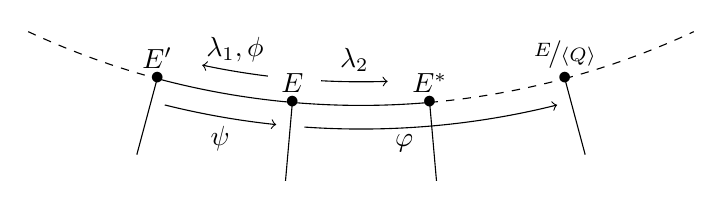
\begin{tikzpicture}[scale=1]
\coordinate (A) at (245:10);
\coordinate (B) at (255:10);
\coordinate (B') at (255:11);
\coordinate (B1) at (256:10.3);
\coordinate (C) at (265:10);
\coordinate (C') at (265:11);
\coordinate (D) at (275:10);
\coordinate (D') at (275:11);
\coordinate (E) at (285:10);
\coordinate (E') at (285:11);
\coordinate (F) at (295:10);
\coordinate (F') at (295:11);
\coordinate (G) at (305:10);
\coordinate (B2) at (258:9.7);
\coordinate (C1) at (266:10.3);
\coordinate (C2) at (267:9.7);
\coordinate (encre) at (273:10.5);
\draw (A) arc(245:255:10)[dashed];
\draw (B) arc(255:275:10);
\draw (D) arc(275:285:10)[dashed];
\draw (E) arc(285:295:10)[dashed];
\draw (B) node[above] {$E'$} node{$\bullet$};
\draw (C) node[above] {$E$} node{$\bullet$};
\draw (D) node[above] {$E^*$} node{$\bullet$};
\draw (E) node[above] {$\nicefrac{E}{\langle Q \rangle }$} node{$\bullet$};
\draw (encre) node {$\varphi$};
\draw (B)--(B');
\draw (C)--(C');
\draw (D)--(D');
\draw (E)--(E');
\draw (B1) arc(256:264:10.3) [->] node[below,midway] {$\psi$}; %flèche représentant \psi
\draw (B2) arc(258:263:9.7) [<-] node[above,midway] {$\lambda_1, \phi$}; %flèche représentant 
\draw (C2) arc(267:272:9.7) [->] node[above,midway] {$\lambda_2$}; %flèche représentant 
\draw (C1) arc(266:284:10.3) [->];% node[below,midway,fill=white] {$\varphi $};

%\draw (260:10.75) node{}
%\draw (0,0) arc (245:255:10)[dashed] node[above] {$C$} node{$\bullet$} --(0:1.5);
%\draw (0,0) arc (245:255:10)[dashed] arc (255:265:10) node[above] {$E^i$} node{$\bullet$} --(0:1.5);
%\draw (-1,0) arc (245:255:10) node[above] {$C2$} node{$\bullet$} --(90:1)[color=yellow];
%\draw (-1,0) arc (245:255:10) node[above] {$C$} node{$\bullet$} --(310:1.5)[color=red];
%\draw (0,0) arc (245:255:10)[color=white] node[above] {$C$} node{$\bullet$} arc (255:265:10) node[above] {$E^i$} node{$\bullet$} arc (265:275:10) node[above] {$E$} node{$\bullet$} arc (275:285:10) node[above] {$F$} node{$\bullet$} arc (285:295:10) node[above] {$G$} node{$\bullet$} ; 
\end{tikzpicture}
\end{center}
\caption{ Example for the case $\ell=2$ } 
\end{figure}

\begin{proof}
%We will first prove that the isogeny $E^* \rightarrow \nicefrac{E^*}{\phi(R)}$ is horizontal and associated to $\lambda_2$.
%\newline
The order of $Q$ is denoted by $\ell^{d_Q}$. Since $\ell \pi(R)=\pi(Q)=\lambda_2Q$ then the $\ell$-isogeny $\psi$ with kernel $\ell^{d_Q}\phi(R)$ is the dual isogeny of $\phi$ because it is the one who anhiliates the $\ell$-torsion on $E$ (here $\langle P, \ell^{d_Q-1}Q \rangle$) together with $\phi$. Thus we have proved that $\psi$ is of direction $\lambda_2$ and horizontal. 
\newline
Since we have $\psi(\phi(R))=Q$, this tells us that the isogeny $\Upsilon$ with kernel $\phi(R)$ is the composition of $\psi$ with the isogeny $\varphi$ of kernel $\langle Q \rangle$. Thus the isogeny $\Upsilon$ is horizontal of degree $\ell^{d_Q+1}$ and associated to $\lambda_2$. 
\end{proof}

After the application of algorithm \ref{Diagnoalizedbasis}, we use the horizontal path of direction $\lambda_2$ we have created by applying it on the point associated to the isogeny of direction $\lambda_1$ to have a generator of an horizontal isogeny of direction $\lambda_1$ on the input curve.%mal formule mais a reformuler...

%Algorithme necessaire, surement pour enfoncer le clou...

\subsection{Proof of the algorithm}
\todo{Dans cette section on montre que une base horizontale est envoyee sur une base horizontale}
Now that we have seen a way to determine a set of $\ell^{\nu_{\ell}(\lambda_1-\lambda_2)+1}$ torsion points, we have to show that this set is invariant under isogenies of degree prime to $\ell$.

\begin{prop}
Let $Q$ be a point of $\ell^j$ torsion with $j>0$ then there exists a division point $V$ of $Q$ of order $\ell^{h+j}$ with $\pi(V)=\lambda_2V$ (or $\pi(V)=\lambda_1V$) if and only if the $\ell^j$ isogeny with kernel $\langle Q \rangle $ is horizontal.
\end{prop}

\begin{proof}
We do a recursive proof. The initial step is the proposition \ref{conjecture}.
\begin{itemize}
\item[$\Leftarrow$]
Recursive step: we consider that the property is true to the rank $j \geqslant 1$.
Let $Q$ be a generator of a $\ell^j$ horizontal isogeny and $V$ a point of order $\ell^{h+j}$ such that $\pi(V)=\lambda_2V$ and $\ell^{h}V=Q$. We consider: $R=\ell^{h-1}V$ a $\ell$ division point of $Q$ and $T$ a division point of $V$ and $\phi$ the $\ell$ isogeny generated by $\ell^{h}P$ with $P$ a point of order $\ell^{h+1}$ such that $\pi(P)=\lambda_1P$. By construction we have $\pi(T)=\lambda_2T + S$ a point of order $\ell$ generator of an isogeny of direction $\lambda_1$, thus with $\phi$ we have $\phi(\pi(T))=\pi(\phi(T))=\lambda_2\phi(T)$, because $\phi$ is a rational isogeny. Since $\phi(R)$ is a generator of a horizontal $\ell^{j+1}$ isogeny by proposition \ref{propcentrale} and  $\ell^h\phi(T)=\phi(R)$  we have proved the recursive step. 
\item[$\Rightarrow$]
Recursive step: we consider that the property is true to the rank $j \geqslant 1$.
Let $Q$ be a point of order $\ell^{j+1}$ with $V$ a division point of $Q$ of order $\ell^{h+1+j}$ with $\pi(V)=\lambda_2V$. We know by hypothesis that the $\ell^j$ isogeny $\phi$ generated by $\langle \ell Q \rangle$ is horizontal. We then have $\phi(Q)$ a point of order $\ell$ and $\phi(V)$ a point of order $\ell^{h+1}$ with $\pi(\phi(V))=\lambda_2\phi(V)$. Thus by applying the proposition \ref{conjecture} we have the isogeny $\psi$ with kernel $\langle \phi(Q) \rangle$ horizontal, therefore the isogeny with kernel $\langle Q \rangle$ that is equal to the composition of $\psi$ with $\phi$ is horizontal.
\end{itemize}
\end{proof}

\begin{prop}
For $\phi$: $E \rightarrow E'$ a $r$-isogeny  with $r \wedge \ell=1$ a prime, and $P$ a $\ell^i$ primitive torsion point, with $i>0$ such that $E \rightarrow E / \langle P \rangle $ is horizontal and $\pi(P)=\lambda_1P$. Then the isogeny  $E' \rightarrow E' / \langle \phi(P) \rangle$ is also horizontal.
\end{prop}

\begin{proof}
We just have to prove that there exists a $\ell^{h+i}$ primitive torsion point $V$ dividing $\phi(P)$ such that $\pi(V)=\lambda_1V$.
Since $P$ is a point that generates a horizontal isogeny then there exists a point $R$ of order $\ell^{h+i}$ dividing $P$. Since $\phi$ is a $r$ isogeny then $\phi$ doesn't change the order of $P$ and $R$, moreover the frobenius commutes with $\phi$ (because this one is defined on $\mathbb{F}_q$) then we have $\pi(\phi(R))=\lambda_1\phi(R)$ which proves the assertion.
\end{proof}

%%%%%%%%%%%%%%%

\section{Interpolation step}
\label{sec:interpolation}
\todo{Dans cette section on montre les outils employes pour diminuer le cout de l interpolation}
Since we consider for the interpolation points on which the Frobenius does not act trivially, we will work only with points that are in different orbits under the action of the Frobenius. As the size of the orbits are not always the same we will have to consider the different orders and combine them efficiently.

\begin{defi}
We will denote by $o_A=max(o_{\lambda_1},o_{\lambda_2})$ and $o_B=min(o_{\lambda_1},o_{\lambda_2})$ with $o_{\lambda_i}$ the order of the eigenvalue $\lambda_i$ in $\mathbb{Z}/\ell^k\mathbb{Z}$. 
\end{defi}

Now we will define polynomials: $\mathcal{T}_i$ that vanish on generator of the orbits of order $o_A$ $o_B$ and the orders $o_A < o_j=\frac{o_A}{\ell^j} < o_B$. Then with the action of the Frobenius we will get the interpolation polynomials defined on all the orbit. We start by taking into account the greatest orbit of order $o_A$ and then we make act the frobenius on this polynomial, we take then into account the next greater order together with the previous polynomial obtained and we repeat this until we get to the order $o_B$.
\newline
Since at each step we obtain a new interpolation polynomial $\mathcal{A}_j$ from the CRT of two other polynomials, and that the modulus do not change at each interpolation try of the algorithm we pre compute the inverse coefficients to fasten the next CRT computation.

\begin{algorithm}
\caption{\label{computingT2ir}Computing $A,T$ other occurrence}
\begin{algorithmic}[5]
\REQUIRE $Lc$ the list with the pre computed inverse for the CRT. All the polynomials $\mathcal{T}_i$.
\ENSURE $T$
\STATE \textit{Compute} $\mathcal{A}_A$ %\STATE $\left( \pi^{o_A/2}(\mathcal{T}_A),\pi^{o_A/2}(\mathcal{A}_A) \right) \gets \left( \mathcal{T}_A,\mathcal{A}_A \right) \in \mathbb{F}_q^{o_A}[x]$
\STATE $\left( R,T \right) \in \mathbb{F}_{q^{o_A/\ell}}[x] \gets CRTs \left( \pi^{o_A/\ell}(\mathcal{A}_A) \bmod  \pi^{o_A/\ell}(\mathcal{T}_A),\mathcal{A}_A \bmod \mathcal{T}_A,Lc(0)(0),Lc(0)(1) \right)$
\FOR{$r=1$ to $\nu_\ell(\frac{o_{A}}{o_{B}})$}%\STATE $\left( R_2=\pi(R)^{o_A/2^{1+r}} T_2=\pi(T)^{o_A/2^{1+r}} \right) \gets \left( R,T \right) \in \mathbb{F}_{q^{o_A/(2^r)}}$
\STATE $\left( R , T \right) \in \mathbb{F}_{q^{o_A/(\ell^{r+1})}}[x] \gets CRTs \left( \pi(R)^{o_A/\ell^{1+r}} \bmod \pi(T)^{o_A/\ell^{1+r}}, R \bmod T,Lc[r][0][0],Lc[r][0][1] \right) $
\STATE \textit{Compute} $\mathcal{A}_r$%\STATE $\left( \pi^{o_A/2^{1+r}}(\mathcal{T}_r), \pi^{o_A/2^{1+r}}(\mathcal{A}_r) \right) \gets \left( \mathcal{T}_r , \mathcal{A}_r \right) \in \mathbb{F}_{q^{o_A/(2^r)}}$ 
\STATE $\left( B,TB \right)\in \mathbb{F}_{q^{o_A/(\ell^{r+1})}}[x]  \gets CRTs \left( \pi^{o_A/\ell^{1+r}}(\mathcal{A}_r) \bmod \pi^{o_A/\ell^{1+r}} (\mathcal{T}_r),\mathcal{A}_r \bmod \mathcal{T}_r,Lc[r][1][0],Lc[r][1][1] \right)$
\STATE $\left( R,T \right) \gets CRTs \left(B \bmod TB, R \bmod T, Lc[r][2][0],Lc[r][2][1] \right) $
\ENDFOR
\FOR{$r=1$ to $\nu_\ell(o_B)-1$}%\STATE $\left( R_2=\pi(R)^{o_B/2^{1+r}}, T2=\pi(T)^{o_B/2^{1+r}} \right) \gets \left( R,T \right) \in \mathbb{F}_{q^{o_B/(2^r)}} $
\STATE $\left( R , T \right)\in \mathbb{F}_{q^{o_B/(\ell^{r+1})}} \gets CRTs \left( R \bmod T ,\pi(R)^{o_B/\ell^{1+r}} \bmod \pi(T)^{o_B/\ell^{1+r}}, Lc[\nu_2(o_B)+r][0][0],Lc[\nu_\ell(o_B)+r][0][1] \right)$
\ENDFOR
\RETURN $R,T$
\end{algorithmic}
\end{algorithm}

%%%%%%%%%%%%%%%

\section{Complete algorithm}
\label{sec:complete-algorithm}
\todo{Put pieces together: explain the strategy for the case where the
  curves are not on the crater, characterize cases where the algorithm
  works/doesn't work, state overall complexity.}
  
  \subsection{Curves which are not on the cyclic crater}

If the input curves of the algorithm are not on a cyclic crater of a volcano of $\ell$-isogeny, but at some level below in the volcano then we can reduce our problem to that case. First we prove that they are located at the same level in the volcano, then we prove that the isogenous curve on the crater are still $r$ isogenous. Then we reduce our problem by determining the shortest path of $\ell$-isogenies that go to the crater of the volcano. For this we can use methods like in \cite{DBLP:journals/amc/MiretMSTV06} or methods that take advantage of the $\ell$-torsion structure if the volcano is regular from \cite{DBLP:journals/moc/MiretMRV05}.
  
\begin{prop}
Let $E_1$ and $E_2$ two elliptic curves $r$-isogenous, with $r$ a prime different from $\ell$. Then they are at the same level in the volcano of $\ell$ isogeny.
\end{prop}

\begin{proof}
We denote by $\mathcal{O}_1$ (resp. $\mathcal{O}_2$) the endomorphism ring associated up to isomorphism to the elliptic curve $E_1$ (resp. $E_2$). Since $E_1$ and $E_2$ are $r$ isogenous we have $[\mathcal{O}_1:\mathcal{O}_2]=f$ with $f \in \{r^1,r^0,r^{-1}\}$ (see Kohel). Moreover we have $[\mathcal{O}_K:\mathcal{O}_2]=[\mathcal{O}_K:\mathcal{O}_1][\mathcal{O}_1:\mathcal{O}_2]$ thus we have $\mathcal{O}_1$ and $\mathcal{O}_2$ at the same level in the volcano of $\ell$ isogeny.
\end{proof}  

For the following results we need to work with elliptic curves defined on $\mathbb{C}$ we use then Deuring theorem to apply those results on elliptic curves defined over finite fields.
We consider $E$ an elliptic curve defined on $\mathbb{C}$ and the $\mathbb{Z}$ lattice associated to $E$ through the Weierstrass $\mathfrak{p}$-function $L=[1,\tau]$ with $\tau$ such that $Im(\tau)>0$(i.e. $\tau \in \mathbb{H}$). We can restrict ourselves to this case up to isomorphism because the $j$-function : $\mathbb{H} \rightarrow \mathbb{C}$ is surjective. Let $\ell$ a prime we denote by
$C(\ell)=\{\left(\begin{array}{cc}
a & b\\
0 & d
\end{array}\right): ad= \ell,0\leqslant b <d, gcd(a,b,d)=1\}$
 For $\sigma \in C(\ell)$, $d[1,\sigma \tau_1]$ is the lattice associated to an $\ell$ isogenous curve of $E_1$ (see Theorem 11.23 and Lemma 11.24 \cite{Cox89}). Thus we can associate $\sigma \in C(r)$ to $r$ isogeny.



\begin{lem} 
Let $E$ be an elliptic curve with the $\mathbb{Z} $ lattice $[1,\tau ]$ associated to $E$ such that $E$ is not on the crater of a volcano of $\ell$ isogeny, then the elliptic curve associated to the $\mathbb{Z}$ lattice $ [ 1, \ell \tau_1 ] $ is the codomain of the $\ell$ ascending isogeny starting from $E$. 
\end{lem}

\begin{proof}
%We consider a $\mathbb{Z}$-basis of the endomorphism ring $[1,\omega_1]$ associated to the elliptic curve $[1,\tau_1]$ since the curve is not on the crater of the volcano we know that $\ell | \omega_1$. 
%\newline
The $\ell$-isogenous curves of $E$ are associated to the lattices $\ell[1,\frac{\tau_1+k}{\ell}]$ with $k \in [0..\ell-1]$ and the lattice $[1,\ell \tau_1]$. Now we consider $\alpha \in \mathrm{End}([1,\tau_1])$ such that $\mathrm{End}([1,\tau_1])= \mathbb{Z} + [\mathcal{O}_K:\mathcal{O}]\mathcal{O}_K=\mathbb{Z}[\alpha]$, by hypothesis we have $\ell | [\mathcal{O}_K:\mathcal{O}]$, we can express $\alpha = a + b \tau_1$ with $a,b \in \mathbb{Z}, a \wedge b =1$, we thus have $\ell \mid \alpha$ and $\ell \mid b$. From the work of Kohel \cite{Kohel} we know that $\alpha$ will be included in only one of the $\ell$ isogenous curve. Since $\alpha \in \mathrm{End}([1,\ell\tau_1]) $ is equivalent to $\ell | b$, we can conclude.
\end{proof}

\begin{prop}
Let consider $\phi : E_1 \rightarrow E_2$ be an isogeny of degree $r$ between the elliptic curves $E_1$ and $E_2$ with $r$ prime different from $\ell$, we denote by $E_{1u}$ (resp. $E_{2u}$) the elliptic curve which is $\ell$ isogenous to $E_1$(resp. $E_2$) and $1$ level above in the volcano(i.e. codomain of an ascending isogenies of degree $\ell$ starting from $E_1$ (resp. $E_2$)). Then $E_{1u}$ and $E_{2u}$ are also $r$-isogenous.
\end{prop}

\begin{proof}
Let consider $\tau_1$ (resp. $\tau_2$)  such that $[1,\tau_1]$ (resp. $d[1,\tau_2]$) is associated to $E_1$ (resp. $E_2$), with $\tau_2=\sigma \tau_1 =\frac{a\tau_1+b}{d}$ and $\sigma =\left(\begin{array}{cc}
a & b\\
0 & d
\end{array}\right) \in C(r)$. 
\newline
By the previous lemma we have the curve $E_{1\mathrm{u}}$ associated to $[1,\ell \tau_1]$ and the curve $E_{2\mathrm{u}}$ associated to $d[1,\ell \tau_2]$.
\newline
We have $\ell \tau_2=\frac{\ell a\tau_1+\ell b}{d}$, since $\forall k \in \mathbb{N}$ $[1,\frac{\ell a\tau_1+\ell b}{d}]=[1,\frac{\ell a\tau_1+\ell b-kd}{d}]$ we can consider that we have $0 \leqslant \ell b<d$.
We set $a'=a, b'=\ell b, d'=d$ wich defines us $\sigma' \in C(r)$ with $\sigma'(\ell \tau_1)=\frac{a'\ell \tau_1+ b'}{d'}=\frac{\ell a\tau_1+\ell b}{d}=\ell \sigma(\tau_1)$. By Theorem 11.23 and Lemma 11.24 of \cite{Cox89} we can then conclude that the curve $E_{1u}$ associated to $[1,\ell \tau_1]$ is $r$ isogenous to the curve $E_{2\mathrm{u}}$ associated to $d[1,\ell \tau_2]$. The case where $E_2$ is associated to $[1,r\tau_1]$ is left to the reader. %easy
\end{proof}
 We can then conclude recursively to obtain the result for curves on the crater.




%%%%%%%%%%%%%%%

\section{Experimental results}
\label{sec:implem}

\todo{Describe implementation and show benchmarks. Possibly compare
  with Lercier-Sirvent (Luca has an implementation somewhere).}

\bibliographystyle{plain}
\bibliography{refs}

\end{document}
